\documentclass{article}
\usepackage{bm}
\usepackage{amsmath}
\usepackage{graphicx}
\usepackage{mdwlist}
\usepackage[colorlinks=true]{hyperref}
\usepackage{geometry}
\usepackage{kotex}
\geometry{margin=1in}
\geometry{headheight=2in}
\geometry{top=2in}
\usepackage{palatino}
%\renewcommand{\rmdefault}{palatino}
\usepackage{fancyhdr}

\newcommand{\red}[1]{{\color{red} #1}}
\newcommand{\blue}[1]{{\color{blue} #1}}
\newcommand{\orange}[1]{{\color{orange} #1}}
\newcommand{\purple}[1]{{\color{purple} #1}}

%\pagestyle{fancy}
\rhead{}
\lhead{}
\chead{%
  {\vbox{%
      \vspace{2mm}
      \large
      Hardware System Design 4190.309A\hfill
\\
      Seoul National University
      \\[4mm]
      \textbf{Practice \#8. OS + FPGA system}\\
      \textbf{Jiwon Lee, Sangjun Son}
    }
  }
}

%%%%%%%%%%%%%%%%%%%%%%%
\usepackage{xcolor}
\usepackage{listings}
\definecolor{vgreen}{RGB}{104,180,104}
\definecolor{vblue}{RGB}{49,49,255}
\definecolor{vorange}{RGB}{255,143,102}

\lstdefinestyle{c-style}
{
    language=C,
    basicstyle=\scriptsize\ttfamily,
    keywordstyle=\color{vblue},
    identifierstyle=\color{black},
    commentstyle=\color{vgreen},
    numbers=left,
    numberstyle=\tiny\color{black},
    numbersep=10pt,
    tabsize=8,
    moredelim=*[s][\colorIndex]{[}{]},
    literate=*{:}{:}1
}

\makeatletter
\newcommand*\@lbracket{[}
\newcommand*\@rbracket{]}
\newcommand*\@colon{:}
\newcommand*\colorIndex{%
    \edef\@temp{\the\lst@token}%
    \ifx\@temp\@lbracket \color{black}%
    \else\ifx\@temp\@rbracket \color{black}%
    \else\ifx\@temp\@colon \color{black}%
    \else \color{vorange}%
    \fi\fi\fi
}
\makeatother

\usepackage{trace}
%%%%%%%%%%%%%%%%%%%%%%%

\usepackage{paralist}

\usepackage{todonotes}
\setlength{\marginparwidth}{2.15cm}

\usepackage{tikz}
\usetikzlibrary{positioning,shapes,backgrounds}

\begin{document}

\pagestyle{fancy}

\section*{Goal}

\begin{itemize*}
\item Implement block design \& execute in zedboard.
\begin{itemize*}
\item Running Debian Linux on zedboard.
\item Running a sample C program.
\end{itemize*}
\end{itemize*}
\begin{figure}[ht]
	\centering
	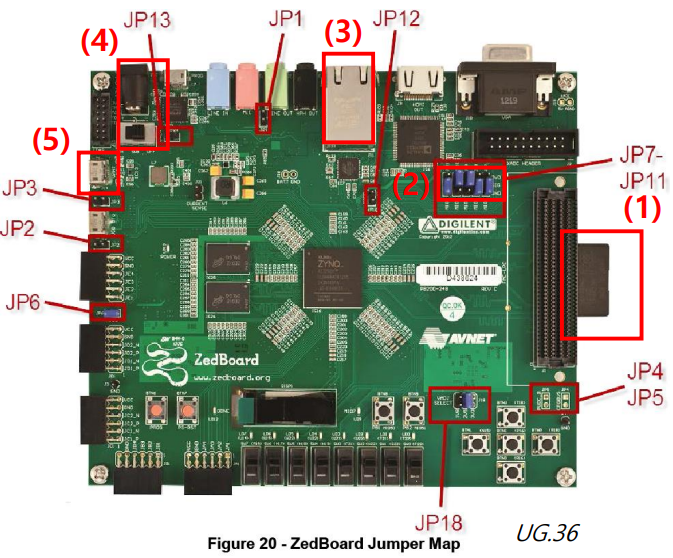
\includegraphics[width=0.6\textwidth]{fig/zedboard.PNG}
\caption{이번 실습에서 사용한 Zedboard. 이전 세션과는 달리 보드를 호스트로 사용하여 실습을 진행한다. 사각형으로 표시된 부분을 유선으로 연결하여 보드 환경을 만들어 주었다. }
\label{fig1}
\end{figure}

\section{Implementation}
이번 프로젝트는 Vivado block design을 사용하여 FPGA위에 Processing System과 Bram을 적절히 연결하여 올리는 Bitstream 파일을 만들었다.
만들어진 Bitstream 파일을 SD 카드에 저장 후 Figure~\ref{fig1}의 (1)에 해당하는 SD 카드 슬롯에 삽입하고 (2)의 SD boot mode를 01100으로 설정해주면 Zedboard 자체를 호스트로 사용할 수 있다. OS (\textit{Linux debian-zynq 4.0.0-xilinx})를 부팅하고, 그 위에서 Zedboard의 주변장치들을 사용할 수 있다~\cite{lab}.\\

특히, block design을 통하여 BRAM과 이외의 custom IP를 사용할 수 있고, 이를 C의 \texttt{mmap}함수를 통하여 실제로 사용해 본다. 
기 주어진 Bitstream 파일을 이용해 실제로 FPGA에서 동작 시켜보고 주어진 \texttt{main.c}을 이용해 Figure~\ref{fig2}의 모듈 \texttt{MyIP}가 어떤 일을 하는지 확인해보았다.

\newpage
\subsection{About \ \texttt{main.c}}
\begin{figure}[ht]
	\centering
	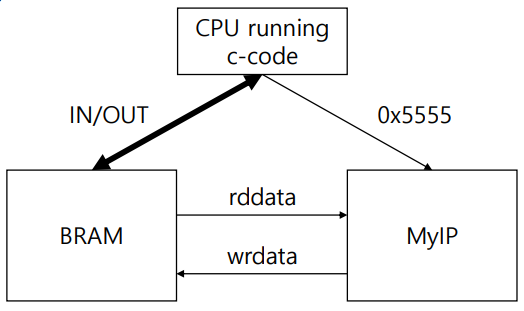
\includegraphics[width=0.5\textwidth]{fig/program_arch.PNG}
\caption{C program에서 사용되는 BRAM과 Custom IP의 아키텍쳐~\cite{lab}}
\label{fig2}
\end{figure}

CPU와 BRAM, IP (unknown)으로 구성되어 있고, IP는 BRAM의 데이터를 읽고, BRAM에 데이터를 써주는 역할을 한다는 것을 알 수 있다. 아래는 실습을 위해 주어진 \texttt{main.c} 소스코드이다.

\subsubsection*{\texttt{main.c}}
\begin{lstlisting}[style={c-style}]
#include <stdio.h>
#include <stdlib.h>
#include <string.h>
#include <fcntl.h>
#include <sys/mman.h>

#define SIZE 4

int main(int argc, char** argv)
{
  int i;

  int foo = open("/dev/mem", O_RDWR);
  int *fpga_bram = mmap(NULL, SIZE * sizeof(int), PROT_READ|PROT_WRITE, MAP_SHARED, foo, 0x40000000);
  int *fpga_ip   = mmap(NULL, sizeof(int), PROT_READ|PROT_WRITE, MAP_SHARED, foo, 0x43C00000);

  // initialize memory
  for (i = 0; i < SIZE; i++)
    *(fpga_bram + i) = (i * 2); 
  for (i = SIZE; i < SIZE * 2; i++)
    *(fpga_bram + i) = 0.0f; 

  printf("%-10s%-10s\n", "addr", "FPGA(hex)");
  for (i = 0; i < SIZE * 2; i++)
    printf("%-10d%-10X\n", i, *(fpga_bram + i));

  // run ip
  *(fpga_ip) = 0x5555;
  while (*fpga_ip == 0x5555);

  printf("%-10s%-10s\n", "addr", "FPGA(hex)");
  for (i = 0; i < SIZE * 2; i++)
    printf("%-10d%-10X\n", i, *(fpga_bram + i));

  return 0;
}
\end{lstlisting}

\begin{itemize*}
\item file descriptor \texttt{foo}를 선언하고, \texttt{mmap}함수를 통해 \texttt{BRAM}, \texttt{IP(unknown)} 를 메모리에 대응시킨다 (13-15라인).\\
\item \texttt{BRAM} memory에 \texttt{BRAM[0]} 부터 \texttt{BRAM[3]}까지는 각각 $(0, 2, 4, 6)$을, \texttt{BRAM[4]}부터 \texttt{BRAM[7]}까지는 \texttt{0.0f(=(int)0)} 을 대응시킨다 (18-21 라인).\\
\item  \texttt{IP(unknown)}에 0x5555를 할당하여 signal을 주고, 다시 \texttt{BRAM}의 메모리를 출력시킨다 (28-33 라인).
\end{itemize*}

\section{Result}
\begin{figure}[ht]
	\centering
	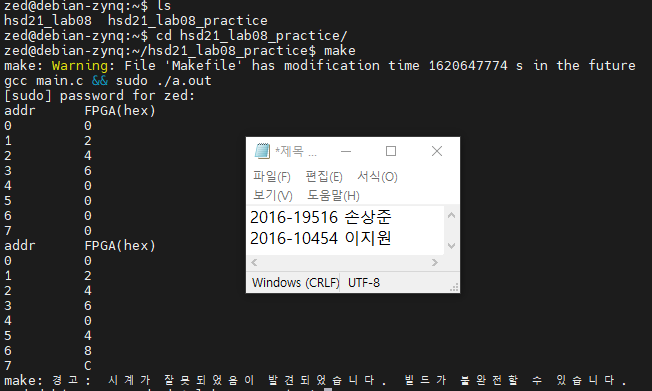
\includegraphics[width=0.6\textwidth]{fig/result.PNG}
\label{fig3}
\caption{\texttt{main.c}를 zedboard에서 실행시켰을 때의 결과화면}
\end{figure}
처음 (MyIP가 수행되기 전) 주소값 (\texttt{addr}) 0-7에 해당하는 BRAM에 저장된 값은 BRAM memory initialization을 수행한 후의 값이고, 두 번째 주소값 0-7에 따른 data값은 IP에 특정 시그널 (\texttt{0x5555})을 주어 이를 실행시킨 후의 값이다. \\

Figure~\ref{fig3}에서 주소 0, 1, 2, 3에 해당하는 BRAM 값이 0, 2, 4, 6으로 잘 초기화 된 것을 확인할 수 있다. 4, 5, 6, 7은 \texttt{while(*fpga\_ip == 0x5555))}가 실행되기 전까지는 0으로 초기화 되었음을 확인하였다. 실행이 된 이후에 주소 4, 5, 6, 7에 해당하는 BRAM값은 0, 4, 8, C로 값이 바뀐 것을 볼 수 있다. 0, 4, 8, C는 0, 2, 4, 6에 2를 곱한 것의 16진수 표현이므로 MyIP가 2를 곱해서 저장해준다고 추론할 수 있다. IP가 실행되고 난 후 결과값을 살펴보았을 때, 주소값 4-7만 바뀌었음을 확인할 수 있고, 다음과 같은 규칙을 가진다고 말할 수 있다.
\begin{equation}
\textrm{BRAM}[i+4] = \textrm{BRAM}[i] \times 2 \quad (0\leq i \leq3)
\label{eqn}
\end{equation}

\texttt{main.c} 에서의 \texttt{fpga\_ip}의 값이 IP input signal이다. \texttt{fpga\_ip}의 값을 바꿔가며 테스트를 했을 때, addr 0-3값은 바뀌지 않고, addr 4-7값만 바뀌었다. 또한, addr 4-7에 0이외의 다른 값들이 있더라도, 기존 값에 위의 수식에서 나온 결과값을 덮어쓰는 것을 확인할 수 있었다. \\

따라서, 프로그램에서 메모리에 매핑된 IP는  multiplier라고 생각하였고, 이 IP는 memory에 있는 BRAM[0-3] 값을 read 하여, 0x5555 signal을 넣어주면, BRAM[0-3] 값을 2배 곱하여 각각 BRAM[4-7] 에 write 해주는 역할을 수행한다. \\

추가적으로, BRAM[0-3]의 초기값을 굳이 \texttt{i*2}의 값으로 초기화하지 않고 다른 값을 입력시켰을 때에도 Equation (\ref{eqn})의 규칙이 성립함을 검증하였다. \texttt{while(*fpga\_ip == 0x5555))}의 값을 다른 값으로 바꾸었을 때 제대로 동작하지 않음을 확인하였다. 이를 통해 MyIP에서 \texttt{0x5555} 외의 다른 값이 주어졌을 때는 기능을 하지 않는다는 사실을 추측할 수 있었다.

\section{Conclusion}
이번 과제에서는 Zedboard 자체를 호스트로 사용하는 것을 실습해보았다. Debian Linux OS가 zynq 버전이 있는 것이 신기하였다. 또한, block design을 vivado에서 수행하고, 이를 OS에 올려 IP들이 돌아가는 과정을 확인할 수 있었는데, 임베디드 시스템의 동작방식도 이와 비슷할 것이라고 생각하였다.

\bibliographystyle{plain}
\bibliography{other}

\end{document}
